\section{Terms and Concepts}



\begin{itemize}
	\item Moving object
	\item Moving region
	\item Fixed-shape moving region
	\item MOD
	\item MobilityDB
\end{itemize}

\section{Moving objects}

There exist a large variety of moving objects. These object can differ in two main ways. Either the type of their value differs, or they are using a different interpolation method.

	\subsection{Value types}

	In theory, for every non-temporal type, there could exist a moving object that extends this type with a temporal dimension. However, in this master thesis, we will only focus on the main types used in this field.

	\begin{itemize}
		\item Scalar types: boolean, string, integer, float
		\item Point types: Either 2d or 3d PostGIS Point types, or network-constrained points called npoints.
		\item Region types: Defined using the PostGIS Polygon type, these regions can either be deforming or fixed-shape.
	\end{itemize}

	\subsection{Interpolation methods}

	Since the values of a moving object are not stored at each time step, intermediate values have to be recomputed using a specific interpolation method. Moving objects with the same value type, but different interpolation methods will thus behave differently and can be considered as different objects. The two main interpolation methods used are:

	\begin{itemize}
		\item Stepwise interpolation (or piecewise constant interpolation): The value of the object does not change between two measurements, but jumps instantly at the time of the next measurement.
		\item Linear interpolation: The value of the object changes linearly between two saved values.
	\end{itemize}

	Discrete value types such as integer or boolean can only use the stepwise interpolation, but continuous types can use both. More complex interpolation methods, such as polynomial or spline interpolation could also be used, but this is not discussed in this work.

	\subsection{Examples}

	\begin{table}[h]
		\centering
		\begin{tabularx}{\textwidth}{
			| >{\raggedright\arraybackslash}X 
  			| >{\raggedright\arraybackslash}X 
  			| >{\raggedright\arraybackslash}X 
			|}
			\hline
			          				& \textbf{Stepwise} 							& \textbf{Linear} 		\\ \hline
			\textbf{Boolean} 		& State of a lightbulb in a room.				&  N/A 				\\ \hline
			\textbf{String} 		& Name of the world record holder for the 100m.	&  N/A       			\\ \hline
			\textbf{Integer} 		& Number of people in a bus.					&  N/A      			\\ \hline
			\textbf{Float} 		& World record time for the 100m.				&  Temperature in a room.		\\ \hline
			\textbf{Point}		& Position of the heighest building in the world	&   Position of players on a court	\\ \hline
			\textbf{NPoint} 		& Position of temporary radars on the side of the road	&   Position of a car       			\\ \hline
			\textbf{Fixed-shape Region} 	& ???	   									&   Movement of a floating city		\\ \hline
			\textbf{Deforming Region} 	& Cadastre         								&   Spread of a forest fire  			\\ \hline
		\end{tabularx}
	\end{table}

\section{Fixed-shape regions}

	In the previous section, the broad range of moving object has been presented. A lot can still be said about these different types of object, however, this thesis is mainly going to focus on diving deeper into the fixed-shape moving regions. These moving regions can generally be represented using simple polygons with zero or more holes. When we talk about a moving fixed-shape polygon, we talk about a certain polygon moving and rotating through time.
	
	\subsection{Representation}

	The first important question that can be asked about fixed-shape moving regions is: how can they be efficiently represented? In the following we will suppose that the polygon is defined at multiple moments in time and we assume that the position of the polygon at intermediate time steps can be found via some kind of interpolation. This is analogous to a moving point (ex: a car), where the position is measured and saved at multiple moments in time, and is supposed to be linearly interpolated. Seeing as the polygon is of fixed shape, storing the position of the polygon at each time step involves storing some redundancy and is thus not really efficient. The first idea is thus to to store the polygon only for the first time step, and then compute and store transformation vectors for the subsequent time steps. This idea has already been explored in \cite{fmregion} and their proposal is to store what they call a transformation unit. This transformation unit is defined between a start instant \( t_s \) and an end instant \( t_e \), and stores the following information.

	\begin{equation}
		T = (C, v_0, v, \theta_0, \theta, t_{s}, t_{e})
	\end{equation}

Where \( v \) is a translation vector and \( \theta \) is an angle. This representation assumes that both the start and the end transformation of the region is stored in the transformation. This is necessary if we suppose that the transformation center can change or if the subsequent transformations are not contiguous to each other. If however we suppose that the transformation center is always the same and that these transformations are contiguous, then there is a lot of redundant information in these transformation units. Since in the standards \note{Maybe more info about the standards?}, there is no mention of the rotation center, and the moving regions are all defined using polygons and not transformations, the rotation center can be chose arbitrarely. Our following supposition is thus that the rotation center of all moving regions is the centroid of the polygon representing the region. Below is a new proposition for the representation of a fixed-shape moving region:

	\begin{equation}
	\begin{split}
		& fmregion = (P_{ref}, [(T_0, t_0), (T_1, t_1), ..., (T_n, t_n)])
	\end{split}
	\end{equation}

	, where \( P_{ref} \) is a simple polygon with zero or more holes, and \( T_i \) is the transformation vector defining the position of the polygon at time \( t_i \). The instants \( t_i \) have to be sorted in increasing order for all \( i \). Since we suppose that the center of rotation is always the centroïd of the polygon defining the region, the information stored in a transformation vector only contains the translation an rotation fo the region. 

	\begin{equation}
	\begin{split}
		& T_{i} = \left ( t_x^{i}, t_y^{i}, \theta^{i} \right )
	\end{split}
	\end{equation}

	In most cases, the position of the polygon at time \( t_0 \) is used as reference polygon, and we have thus \( T_0 = (0, 0, 0) \).

	To compute these transformation vectors starting from two regions at two different time steps, multiple techniques are possible. \cite{fmregion} proposes a way to compute these transformation units that allow for some slight differences between the start and the end region. In the following however, we will suppose that the start and end regions are identical and that the corresponding points on each polygon are known. With this assumption made, it is sufficient to take the center of rotation and one other point of each polygon to compute the transformation. We define the start and end centroids, additional points and transformation vectors as follows:

	\begin{equation}
	\begin{split}
		& C^{i} = (c_{x}^{i}, c_{y}^{i}) \\
		& P^{i} = (p_{x}^{i}, p_{y}^{i}) \; \; \; \; \; i \in \left \{ start, end \right \} \\
		& T^{i} = \left ( t_x^{i}, t_y^{i}, \theta^{i} \right ) \\ 
	\end{split}
	\end{equation}

	Since every transformation is defined relative to a reference polygon, we also need to define this reference polygon. In this example case we will take the start region as being the reference polygon. This means that the start transformation vector will be zero: \( T_{start} = \left ( 0, 0, 0 \right ) \). The transformation vector for the end region can then be computed in the following way. First the translation component is computed by doing the difference between the positions of the start and end centroids.


	\begin{equation}
	\begin{split}
		& t_x^{end} = c_x^{end} - c_x^{start} \\
		& t_y^{end} = c_y^{end} - c_y^{start}
	\end{split}
	\end{equation}

	Then, the end polygon (only the needed point) is moved back to its starting position by cancelling the translation.


	\begin{equation}
	\begin{split}
		& {P^{end}}' = ({p_{x}^{i}}', {p_{y}^{i}}') \\
		& {p_x^{end}}' = p_x^{end} - t_x^{end} \\
		& {p_y^{end}}' = p_y^{end} - t_y^{end} \\
	\end{split}
	\end{equation}

	Finally, the angle between the start and end polygon is computed.

	\begin{equation}
	\begin{split}
		& \theta^{end} = \angle P^{start} C^{start} {P^{end}}' , \; \; \; \theta^{end} \in \left ] - \pi , \pi \right ]
	\end{split}
	\end{equation}

	\subsection{Operations on fixed-shape regions}

	Intro on operations

	List of operations with input to output types

	\begin{itemize}
		\item atinstant/getValue
		\item interpolate
		\item traversed area
		\item point inside
		\item distance?
		\item union or diff ?
	\end{itemize}

		\subsubsection{AtInstant/getValue}
		
		When defining a moving region over a certain time period, it is important to be able to know what the position of the region is at any instant in time during that time period. This is done using the \note{getValue / atInstant?} function. This function takes a moving region and an instant as input and returns the position of the region at that moment in time. To compute this position, we first have to compute the transformation of the region at that moment. When the transformation with respect to the reference region is know, we can just apply this transformation and we obtain the needed region. Applying this transformation to the reference region means applying it to every point of the region.
		With \( P = (p_x, p_y) \) being the start point and \( T = (t_x, t_y, \theta) \) being the transformation, we compute the end point \( P' = ({p_x}', {p_y}')  \) as follows:

		\begin{equation}
		\begin{split}
			& {p_x}' = cos(\theta)*p_x - sin(\theta)*p_y + t_x \\
			& {p_y}' = sin(\theta)*p_x + cos(\theta)*p_y + t_y \\
		\end{split}
		\end{equation}

		The main issue now is to compute the correct transformation for the given instant. Suppose that the position of the region is defined at time steps \( [t_0, t_1, t_2, ..., t_n] \) and that the region is well-defined between these time steps. 

		\begin{equation}
		\begin{split}
			& fmregion = (P_{ref}, [(T_0, t_0), (T_1, t_1), ..., (T_n, t_n)])
		\end{split}
		\end{equation}

		If the given instant is one of the \( t_i \)'s, then the corresponding transformation will be \( T_i \) and the work is done. If the instant is before \( t_0 \) or after \( t_n \), then the region will return an empty region \note{empty or error or null?}, since the region is not defined at that moment. Lastly if the instant is between \( t_i \) and \( t_{i+1} \), then the transformation has to be computed by interpolating between the transformations \( T_i \) and \( T_{i+1} \). This interpolation is explained in the following subsection.

		\subsubsection{Interpolation}

		Suppose that we know the position of a moving region at times \( t_i \) and \( t_{i+1} \) and that we want to know what the position of that region is in between these instants. Since we previously supposed that the respective points of different regions/polygons are known, a first possible interpolation method would be to linearly interpolate each respective vertex of the start and end polygon. An example of this can be seen below. 
		
		\note{Add an example}
		
		\begin{figure}[h]
			\centering
			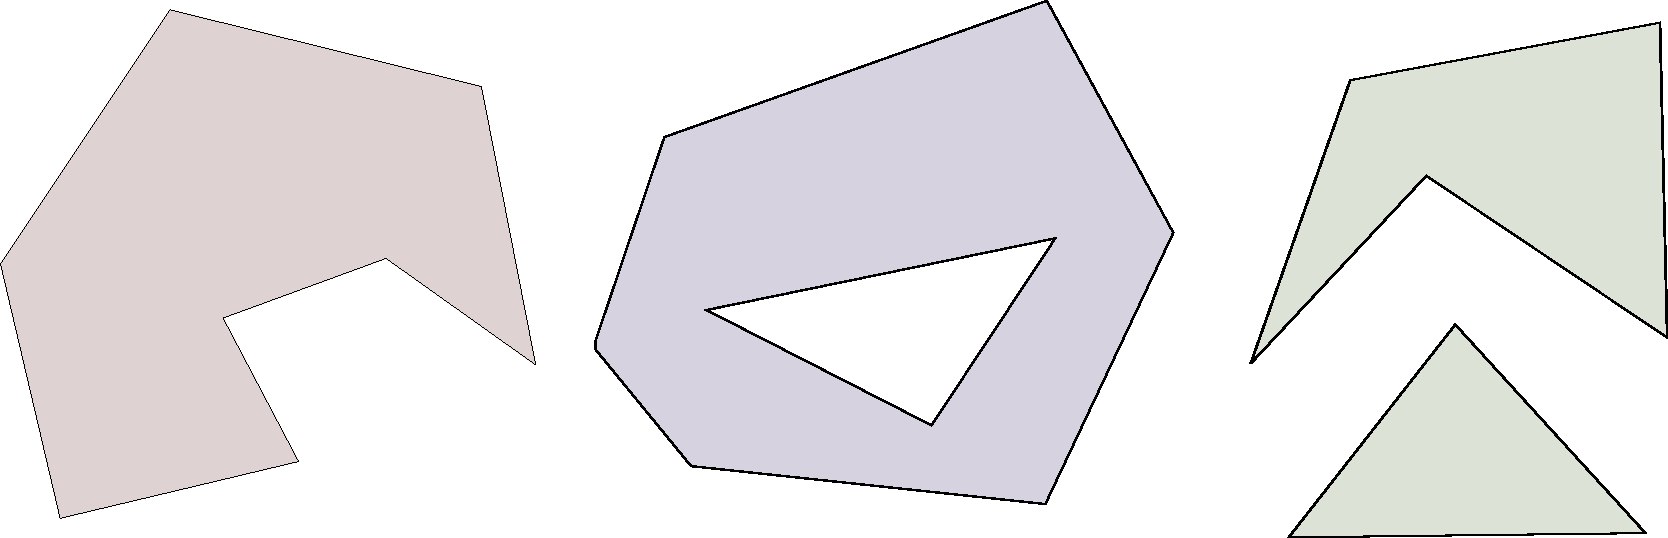
\includegraphics[width=0.9\textwidth]{images/polygons.pdf}
			\caption{Example of a correct linear interpolation of vertices between two regions}
			\label{fig:correct_vertices_interpol}
		\end{figure}
		
		\begin{figure}[h]
			\centering
			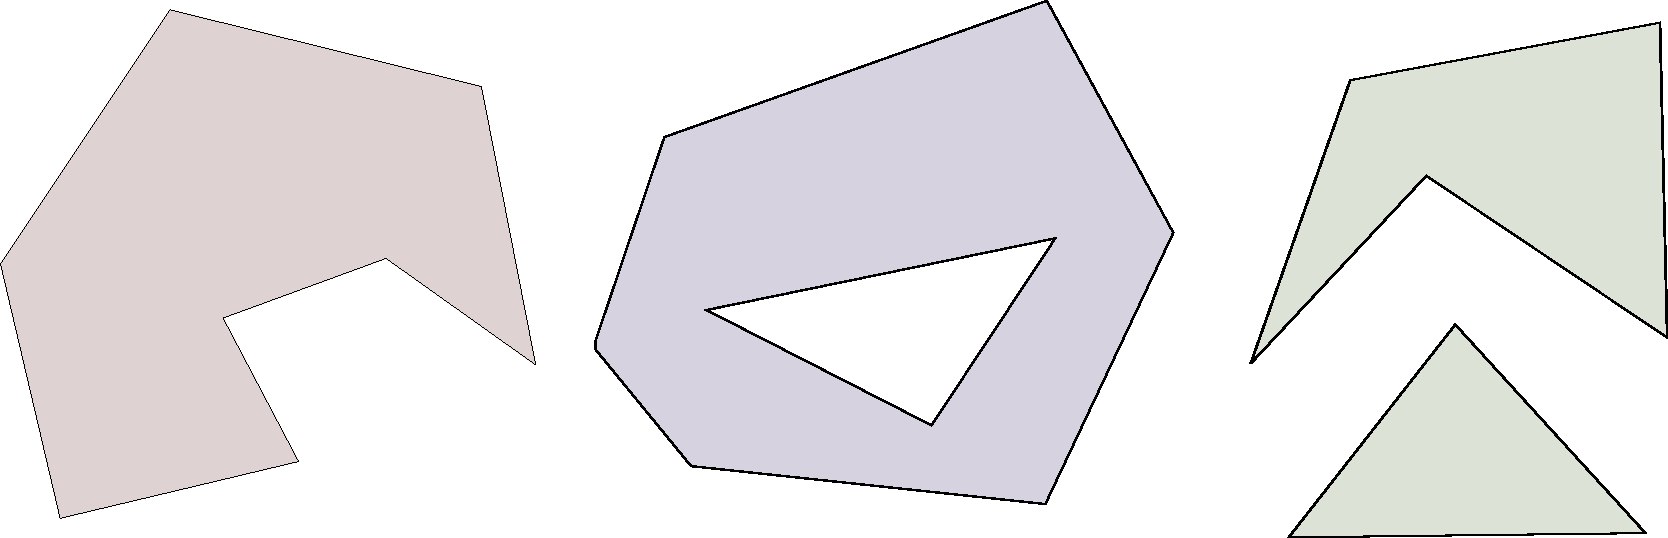
\includegraphics[width=0.9\textwidth]{images/polygons.pdf}
			\caption{Example of a wrong linear interpolation of vertices between two regions}
			\label{fig:wrong_vertices_interpol}
		\end{figure}

		As we see on above example, this seems to work well when the region is only translating. However, when the moving region is also rotating, this interpolation method fails to maintain the fixed-shape aspect of the region, and produces regions that are deforming along the translation. This comes from the fact that this interpolation method assumes that the vertices of the region move freely and independently of each other. For fixed-shape moving region this is unfortunately not the case, so this interpolation method cannot be used when rotations are involved. \note{Add an example}

		The solution for this is to interpolate the transformation instead of the vertices of the region. When applying a transformation (translation + rotation) to a region, the shape of the region will be maintained, which is what we want. To interpolate two transformations, two steps have to be done. First the translation vectors have to be linearly interpolated. Then the rotation has to be interpolated using a spherical interpolation method. For example: suppose that we want the transformation at time \( t_0 < t_i < t_1 \), with the transformations \( T_0 = (t_x^0, t_y^0, \theta^0) \) and \( T_1 = (t_x^1, t_y^1, \theta^1) \) at times \( t_0 \) and \( t_1 \) known. The transformation \( T_i = (t_x^i, t_y^i, \theta^i) \) can then be computed in the following way.

		\begin{equation}
		\begin{split}
			& r = \frac{t_1 - t_i}{t_1 - t_0} \\
			& t_x^i = t_x^0 * r + t_x^1 * (1-r) \\
			& t_y^i = t_y^0 * r + t_y^1 * (1-r) \\	
			& \theta^i = slerp(\theta^0, \theta^1, r) \\
		\end{split}
		\end{equation}

		To compute \( \theta^i \), we have to take into account the fact that we are interpolating an angle and that we want \( \theta^i \in \left ] - \pi , \pi \right ] \). Suppose without loss of generalization that \( \theta^0 <= \theta^1 \) (Otherwise just call \textit{slerp} with the parameters \( slerp(\theta^1, \theta^0, 1-r) \)). Two different cases have to be considered: the case where \( \theta^1 - \theta^0 <= \pi \) and the case where \( \theta^1 - \theta^0 > \pi \). Both cases are illustrated below.
		
		\note{graph with interpolation of angles}

		The \note{red?} portion of the circle corresponds to the values that the interpolated angle can take depending on the value of \( r \). In the first case, a linear interpolation of the angles gives the correct result. In the second case, however, we have to take into account the fact that  both angles are between \( -\pi \) and \( \pi \). The interpolated angle can then be computed by first adding \( 2\pi \) to the smallest angle, interpolating linearly the resulting angles and then substracting \( 2\pi \) from the resulting angle if it is larger than \( \pi \).

		\begin{equation}
		\begin{split}
			\text{case } 1: \, & \theta^i = \theta^0 * r + \theta^1 * (1-r) \\
			\text{case } 2: \, & \theta = (\theta^0 + 2\pi) * r + \theta^1 * (1-r) \\
						   	    & \theta^i = 
									\begin{cases}
										\theta - 2\pi, & \text{if } \theta^i > \pi\\
										\theta,         & \text{otherwise}
									\end{cases}
		\end{split}
		\end{equation}

		This method will give the correct interpolation of regions for transformations in 2d. However, in 3d, Euler angles are hard to interpolate with the same method. There is thus another technique that allows for the interpolation of rotations in both 2d and 3d in a similar manner. This technique uses \textit{quaternions}, and is described in section \note{link to section}.
		
		\subsubsection{TraversedArea}
		\label{section:traversed_area}
		
		\note{Todo}
		
		\subsubsection{PointInside}
		
		\note{Todo}
		
		\subsubsection{Distance}
		
		\note{Todo}
		
		\subsubsection{Union / Diff?}
		
		\note{Todo}
			
	\subsection{Quaternions for interpolation of rotations}
	
	\note{say that no formal definitions or proofs are given and that a more complete definition/explanation of quaternions can be found somewhere else + refs (ex. see paper from mit in favorites)}
	
	Section \note{link to section} describes a basic way to compute the interpolation of a rotation in 2d defined by a single angle. In 3d, however, the angles needed to describe a rotation are the Euler angles, and this method is not well-suited for these angles. \note{note + ref to gimbal lock} Another method for describing rotations in 2d and 3d are rotation matrices. \note{Compared to rotation matrices they are more compact, more numerically stable, and more efficient. - Wikipedia: Quaternions and spatial rotation $\rightarrow$ find source} Lastly, rotations in 3d (and 2d, 4d) can also be described using quaternions, and this technique allows for an easy interpolation method, which will be described later. Althought this master thesis mainly focusses on the moving regions in 2d (since most operations on moving objects are either really easy to generalise to 3d (ex: atInstant) or extremely hard (ex: TraversedArea), so only the 2d version is described \note{Maybe add this note earlier (intro or start of theory)}), since this technique using quaternions works for both 2d and 3d, we are adding this section to allow for an easy generalisation to 3d if needed. A small section is added in the end showing how complex numbers can be used in a similar way to interpolate 2d rotations by using less parameters than quaternions.
	
		\subsubsection{Representing 3d rotations using Quaternions}
		
		Quaternions were first described by William Rowan Hamilton in 1843 \note{citation?} and are an extention to complex numbers. Quaternions are represented in the following way.
		
		\begin{equation}
			q = a + bi + cj + dk, \; \text{with } a, b, c, d \in \mathbb{R} \\
		\end{equation}
		
		The symbols \( i, j \) and \( k \) can be interpreted as unit vectors in a three dimensional space, and are analoguous to the symbol i in complex numbers. Multiplication of complex numbers uses the fact that \( i^2 = -1 \). In a similar way, quaternion multiplication is defined the multiplication rules of \( i, j \) and \( k \) with each other.
		
		\begin{equation}
			i^2 = j^2 = k^2 = ijk = -1 \\
		\end{equation}
		
		These equation above define the complete behaviour of the three symbols, and the equations below can be found using them.
		
		\begin{align*}
			ij &= k & ji &= -k \\
			jk &= i & kj &= -i \\
			ki &= j & ik &= -j \\
		\end{align*}
		
		Quaternion multiplication can then be done similarly to the multiplication of complex numbers by taking into account the multiplication rules for these three symbols. An important thing to note is that quaternion multiplication is not commutative, as can be seen when multiplying quaternions \( q_1 = i \) and \( q_2 = j \): \( q_1*q_2 = ij = k \) and \( q_2*q_1 = ji = -k = -q_1*q_2 \). A unit quaternion is a quaternion of unit length, meaning its norm is equal to 1. 
		
		\begin{equation}
			\left \| q \right \| = \sqrt{a^2 + b^2 + c^2 + d^2}
		\end{equation}
		
		Unit quaternions can be used to efficiently represent orientations or rotations in three dimensions. When a unit quaternion is used to represent a rotation, it is called a rotation quaternion. For example, a rotation of an angle \( \theta \) around the axis \( \vec{v} = (x, y, z) \) can be represented by the rotation quaternion:
		
		\begin{equation}
			q = \cos(\frac{\theta}{2}) + \frac{(xi + yj + zk)}{\sqrt{x^2 + y^2 + z^2}}*\sin(\frac{\theta}{2})
		\end{equation}
		
		Rotating a point/vector \( p = (p_x, p_y, pz_) = p_xi + p_yj + p_zk \) by \( \theta \) around \( \vec{v} = (x, y, z) \) involves evaluating the conjugation of \( p \) by \( q \) 
		
		\begin{equation}
			p' = q*p*q^{-1}
		\end{equation}
		
		, where \( q^{-1} \) is the reciprocal of \( q \), which for unit quaternions is the same as the conjugate of \( q \) since \( q \) is already normalized.
		
		\begin{equation}
		\begin{split}
			q^{-1} & = \frac{q^{\ast}}{{\left \| q \right \|}^2} \\
					& = \frac{\cos(\frac{\theta}{2}) - \frac{(xi + yj + zk)}{\sqrt{x^2 + y^2 + z^2}}*\sin(\frac{\theta}{2})}{{\left \| q \right \|}^2} \\
					& = \cos(\frac{\theta}{2}) - \frac{(xi + yj + zk)}{\sqrt{x^2 + y^2 + z^2}}*\sin(\frac{\theta}{2}) \\
		\end{split}
		\end{equation}
		
		When rotating a point or polygon around an axis that does not go through the origin, we first have to translate the point/polygon to make the rotation axis go through the origin. For example if the axis goes through the centroid of a polygon, we first have to translate this polygon so that its centroid and the origin are coincident. Then, we apply the rotation to each vertex of the polygon. Finally, the polygon is translated back to return its centroid at the inital position.
		
		Multiple rotations can be combined together into a single one by combining the corresponding quaternions. For example, the combined rotation of first applying \( q_1 \) and then \( q_2 \) can be computed like this:
		
		\begin{equation}
		\begin{split}
			q 	& = q_2*q_1 \\
			p' 	& = q*p*q^{-1} \\
				& = (q_2*q_1)*p*(q_2*q_1)^{-1} \\
				& =  (q_2*q_1)*p*(q_1^{-1}*q_2^{-1}) \\
				& = q_2*(q_1*p*q_1^{-1})*q_2^{-1} \\
		\end{split}
		\end{equation}
		
		, which indeed correspond to first applying \( q_1 \) to \( p \) and then applying \( q_2 \) to the previous result.
		
		The efficiency of using quaternions instead of rotation matrices or axis-angle representations can be debated, but the main advantage of using these rotation quaternions is that we can easily apply a spherical linear interpolation (\textit{slerp}) to them. This is necessary to correctly interpolate between two 3d rotations, which is needed for the 3d version of the \textit{interpolate} function described in section \note{link to section}. To use the resulting quaternion to effectively rotate a polygon can be done by either first transforming all polygon vertices to a quaternion representation and then doing quaternion multiplication, or by representing the resulting rotation quaternion in another way, for example using a rotation matrix, and then applying this rotation matrix to the polygon. Transformations from rotation quaternion to other rotation representations has been presented in \cite{ISO19141}, and the equations have also been added in Annex \note{TODO: write annex and add ref to annex}.
			
		\subsubsection{Interpolating 2d and 3d rotations using Quaternions}
		
		Now that rotation quaternions have been presented as a method used to represent 3d rotations, let's look at how we can compute an interpolation between two rotations. An example of the interpolation of two 3d rotations can be seen below. \note{add example} The computations can be done relatively easily using quaternions, and corresponds to a spherical linear interpolation (\textit{slerp}) in 3d.
		
		The interpolation process can be represented mathematically as follows. To interpolate between two rotations represented by quaternions \( q_0 \) and \( q_1 \), we first compute an angle \( \theta \) between them, and then apply the \textit{slerp} process to find the interpolated rotation.
		
		\begin{equation}
		\begin{split}
			\cos(\theta) 	& = q_0 \note{dot} q_1 \\
			q(r) 			& = Slerp(q_0, q_1, r) \\
							& = \frac{q_0 * \sin((1-r)*\theta) + q_1 * \sin(r*\theta)}{\sin(\theta)}
		\end{split}
		\end{equation}
			
		\subsubsection{Interpolating 2d rotations using complex numbers}
		
		We have shown how quaternions can be used to represent 3d rotations and to compute interpolation between 3d rotations. These techniques can thus also be used for 2d rotations, since they are a special type of 3d rotations and the interpolation between two 2d rotations also results in a 2d rotation.
		Nevertheless, using a quaternion rotation for 2d rotations might be overkill if 3d rotations do not need to be handled. A method has previously been described that handles only 2d rotations, but as said previously, it has to handle edge cases, because of the fact that rotation angles have to be between \( - \pi \) and \( \pi \). Another method uses complex numbers to, similarly to the previously mentioned quaternions, compute interpolation of 2d rotations in an efficient way. This is done using the exact same technique as with quaternions, but using less parameters. The equations are shown below, and the similarity with the previously defined equations for quaternions can clearly be seen.
		
		A rotation of $\theta$ around the origin can be represented using the complex number \( q = \cos(\frac{\theta}{2}) + i*\sin(\frac{\theta}{2}) \) and a 2d point \( p = (x, y) \) can be represented using the complex number \( p = x + i*y \). Computing the interpolation between two rotations \( q_0 \) and \( q_1 \) can be done in a similar manner as quaternion interpolation.
		
		\begin{equation}
		\begin{split}
		\cos(\frac{\theta}{2})	&= q_0 \note{dot} q_1 \\
								&= \cos(\frac{\theta_0}{2})*\cos(\frac{\theta_1}{2}) + \sin(\frac{\theta_0}{2})*\sin(\frac{\theta_1}{2}) \\
								&= \cos(\frac{\theta_1 - \theta_0}{2}) \\
								& \\
		q(r)				&= Slerp(q_0, q_1, r) \\
						&= \frac{q_0 * \sin((1-r)*(\frac{\theta}{2})) + q_1 * \sin(r*(\frac{\theta}{2}))}{\sin((\frac{\theta}{2}))} \\
						&= \cos((1-r)*\frac{\theta_0}{2} + r*\frac{\theta_1}{2}) + i*\sin((1-r)*\frac{\theta_0}{2} + r*\frac{\theta_1}{2}) \\
		\end{split}
		\end{equation}
		
		and the same can be said for applying the rotation to an arbitrary point.
		
		\begin{equation}
		\begin{split}
			p' 	&= q*p*q \\
				&= q^2*p \\
				&= (\cos(\frac{\theta}{2})^2 + \sin(\frac{\theta}{2})^2 + i*2\cos(\frac{\theta}{2})\sin(\frac{\theta}{2}))*p \\
				&= (\cos(\theta) + i*\sin(\theta))*(x + i*y) \\
				&= (x*\cos(\theta) - y*\sin(\theta)) + i*(x*\sin(\theta) + y*\cos(\theta)) \\
		\end{split}
		\end{equation}
			










